\subsubsection{GodkendelsesTabel Game Engine}
Nedestående præsenteres en fuld tabel for alle classes testet som 
led i Game Engine. De vigtigste er GameController, CombatController,
Player/Room og DiceRoller. Dice danner ``Core Mechanics'' for spillet.

Interessant nok ses her at GameController fejler sine test grundet at
der ikke er skrevet test til mange af GameControllerens ansvars punkter.

\begin{center}
\captionof{table}{Her Ses en komplet liste over alle test foretages på
                  Game Engine komponenter, med kommentar til deres resultater
                  og en endelig vurdering af test resultaterne.}
\vspace{-1em}
\label{tab:testEngine}
  \begin{longtable}{|l|p{0.25\linewidth}|p{0.25\linewidth}|l|}
  \hline
  \multicolumn{4}{|c|}{\textbf{Game Engine GodkendelsesTabel}} \\ \hline
  \textbf{Komponent under test} & \textbf{Forventet Adfærd} & \textbf{Kommentar} & \textbf{Test Resultat} \\ \hline
  Game Controller
  &
    \begin{enumerate}
      \item \begin{flushleft} Kan skifte Player til Nyt Room \end{flushleft}
      \item \begin{flushleft} Kan samle Item op fra Room  \end{flushleft}
      \item \begin{flushleft} Kan save Game \end{flushleft}
      \item \begin{flushleft} Kan loaded Games \end{flushleft}
      \item \begin{flushleft} Kan eliminere Enemy fra Game \end{flushleft}
      \item \begin{flushleft} Kan reset Game \end{flushleft}
      \item \begin{flushleft} Kan anskaffe Room description \end{flushleft}
    \end{enumerate}
  &
  \flushleft 
  Game Controller er kun test for at skifte til nyt Room, dette betyder at der 
  ikke kan stilles garanti for at resterende implementeringer af load- og save game
  osv. fungere som ønsket. Disse ting er svagt testet gennem visuelt trial and error
  test, men da der ikke er skrevet nogen specifikke test til dem Fejler 
  GameControlleren sin komponent test.
  &
  FAIL
  \\ \hline
  Combat Controller
  &
  \begin{enumerate}
    \item \begin{flushleft} Kan Håndtere Combat Rounds \end{flushleft}
    \item \begin{flushleft} Kan håndtere at Player løber væk fra Combat \end{flushleft}
  \end{enumerate}
  &
  \flushleft
  Combat controller kan håndtere at spilleren løber fra combat og at Player indgår i combat.
  CombatController kan stille garanti for at combat sker i den rigtige orden og at hverken
  spiller eller enemy kan angribe hvis denne er død.
  Ydmere stiller den garanti for at både enemy og spiller kan lave ``critial hits'' hvis dice
  rolleren slår 20.
  &
  OK
  \\ \hline
  DiceRoller
  &
  \begin{enumerate}
    \item \begin{flushleft} Kan emulerer et kast med en N siddet terning \end{flushleft}
    \item \begin{flushleft} Kan emulerer N kast med en M siddet terning \end{flushleft}
  \end{enumerate}
  &
  \flushleft
  DiceRoller Kan emulere et eller flere terninge kast med samme antal sidder. Denne kan
  ydmere stille krav for at fordellingen af disse terningekast har en normal distribution 
  og dermed er alle udfald lige sandsynlige.
  &
  OK
  \\ \hline
  BaseMapCreator
  &
  \begin{enumerate}
    \item \begin{flushleft} Kan generere et map layout file \end{flushleft}
  \end{enumerate}
  &
  \flushleft
  BaseMapCreator can på korrekt vis generere et map layout file, den kan ydmere
  generer item layout files og Enemy layout files, der hjælper Map klassen med 
  at genererer spillet Map. Der ikke skrevet test for eksistensen af item og enemy 
  layout Map og derfor kan der ikke stille garanti for at disse bliver genereret 
  på korrektvis. Testen Fejler derfor.
  &
  FAIL
  \\ \hline
  BaseMap
  &
  \begin{enumerate}
    \item \begin{flushleft} Kan anskaffe Rooms ud fra en Direction \end{flushleft}
  \end{enumerate}
  &
  \flushleft
  Map kan anskaffe Rooms uf fra en given Direction. Map kan på korrektvis generer et 
  map udfra mappets layout file. Den kan også på korrektvis finde udaf hvilke Rooms
  har adgang til hinanden. Der er ikke skrevet test for at bekræfte at enemy og items er 
  i de korrekte lokationer baseret på enemy og item layout filerne.
  Derfor fejler denne sin Test.
  &
  FAIL
  \\ \hline
  Player
  &
  \begin{enumerate}
    \item \begin{flushleft} Kan angribe Enemy  \end{flushleft}
    \item \begin{flushleft} Kan tage skade \end{flushleft}
    \item \begin{flushleft} Kan skade Enemy (Ikke Kristisk)  \end{flushleft}
    \item \begin{flushleft} Kan skade Enemy (Kritisk)  \end{flushleft}
  \end{enumerate}
  &
  \flushleft
  Player kan angribe, skade og tage skade fra enemy. 
  &
  OK
  \\ \hline
  Enemy
  &
  \begin{enumerate}
    \item \begin{flushleft} Kan angribe Player  \end{flushleft}
    \item \begin{flushleft} Kan tage skade \end{flushleft}
    \item \begin{flushleft} Kan skade Player (Ikke Kristisk)  \end{flushleft}
    \item \begin{flushleft} Kan skade Player (Kritisk)  \end{flushleft}
  \end{enumerate}
  &
  \flushleft
  Enemy kan angribe, skade og tage skade fra Player.
  &
  OK
  \\ \hline
  Log
  &
  \begin{enumerate}
    \item \begin{flushleft} Kan log et event \end{flushleft}
    \item \begin{flushleft} Kan anskaffe et event \end{flushleft}
    \item \begin{flushleft} Kan merge to logs \end{flushleft}
  \end{enumerate}
  &
  \flushleft
  Log kan logge et event, anskaffe eventet og merge to forskellige logs.
  &
  OK
  \\ \hline
  Room                          
  & 
  \begin{enumerate}
    \item Kan tilføje Player
    \item Kan tilføje Enemy
    \item Kan fjerne Player
    \item kan fjerne Enemy
  \end{enumerate}
  &
  \flushleft
  Room kan fjerne/tilføje Player og Enemy som forventet
  &
  OK
  \\ \hline
  Items
  &
  \begin{enumerate}
    \item[]
  \end{enumerate}
  &
  \flushleft
  Items så som sword, shield, axe osv.\ indeholder kun data og har derfor ikke nogen
  testbar adfærd andet end deres constructor. De kan alle construeres på korrekt vis.
  &
  OK
  \\ \hline
\end{longtable}
\addtocounter{table}{-1}
\end{center}

\newpage 

\subsubsection{Mock testing}
I nogle tilfælde kan det være umuligt er lave troværdige tests, når
en klasse f.eks. Player er dyb afhængig af DiceRoller klassen. Dette skyldes
at DiceRoller danner pseudo-random outputs og derfor er test med den ikke 
altid troværdige.

Her benyttes mock tests og dependency injections til at sikre at DiceRoller 
klassen danner de samme outputs hver gang en test køres.
Derved kan alle senarier for Player klassen testes, hvor man kan regne med at DiceRoller giver et bestemt output. 

\begin{figure}[H]
  \centering
  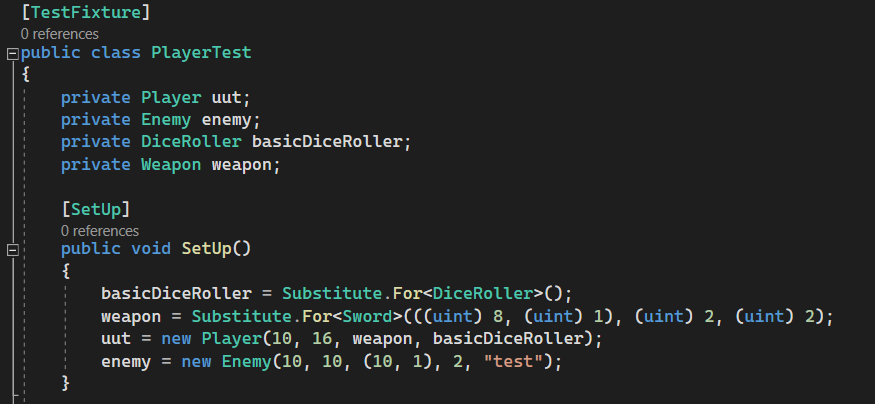
\includegraphics[scale=0.5]{02-Body/Images/Mocks_And_Dependency_Injection.png}
    \caption{}
  \label{fig:mock}
\end{figure}

\begin{figure}[H]
  \centering
  \includegraphics[scale=0.45]{02-body/Images/useofmocks.png}
    \caption{Mocks benyttes her til at sikre at dependencien, her DiceRoller, returner
           den ønskede værdi for situationen, der er under test.
           Alle test tildeles informative navne, for at sikre læsbarhed i forhold 
           til testenes formål.}
  \label{fig:mockuse}
\end{figure}

\newpage 

\subsubsection{Test Resultater for Game Engine}
Nedestående vises kort resultatet for Game Engine test, når de alle køres via visual studio. Som det kan ses så er alle testene succesfulde, hvilket giver hvis garanti for at
game engine opfører sig som specificeret i kravspecifikationerne og i de implementerede interfaces.

\begin{figure}[H]
  \centering
  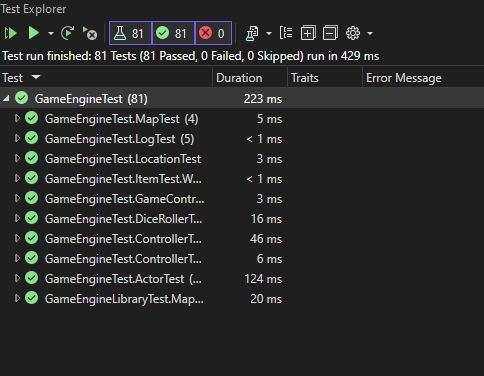
\includegraphics[scale=0.4]{02-body/Images/Test Results.png}
    \caption{Alle skrevene test til Game Engine passer, hvilket hjælper med at give vished
          om at Game Engine udfører dens funktionalitet, som det er beskrevet i kravene.
          Dette siges da alle testene er skrevet på baggrund af kravene som black-box tests
          og ikke som white-box test efter implementeringen.}
  \label{fig:TestResultsGameEngine}
\end{figure}



